\documentclass[a4paper]{article}
\usepackage{amsmath,amssymb,amsfonts,amsthm}
\usepackage{multicol}
\usepackage{multirow}
\usepackage{mathtools}
\usepackage{soul}
\usepackage{hyperref}
\hypersetup{
    colorlinks=true,
    linkcolor=blue,
    filecolor=magenta,      
    urlcolor=cyan,
    pdftitle={Overleaf Example},
    pdfpagemode=FullScreen,
    }
\usepackage{color}
\usepackage[table]{xcolor}
\usepackage[T1]{fontenc}
\usepackage{etoolbox}
\usepackage{multicol}
\usepackage{multirow}
\usepackage{fancyhdr}
\usepackage{graphicx}
\usepackage{array}
\usepackage{amsthm}
\usepackage{titlesec}
\usepackage{tikz}
\usepackage{pgfplots}
\pgfplotsset{compat=1.18}
\usetikzlibrary{arrows.meta,calc}
\renewcommand{\baselinestretch}{1.2}

\titleformat*{\section}{\large\bfseries}
\titleformat*{\subsection}{\normalsize\bfseries}

\graphicspath{{C:/Users/teoso/OneDrive/Documents/Tugas Kuliah/Template Math Depart/}}

\newtheorem{theorem}{Theorem}
\newtheorem*{teorema}{Teorema}
\newtheorem*{definisi}{Definisi}
\theoremstyle{definition}
\newtheorem*{bukti}{Bukti}
\newtheorem*{solusi}{Solusi}
\newtheorem*{contoh}{Contoh}

\newcommand{\Arg}{\text{Arg}}
\newcommand{\N}{\mathbb{N}}
\newcommand{\Z}{\mathbb{Z}}
\newcommand{\Q}{\mathbb{Q}}
\newcommand{\R}{\mathbb{R}}
\newcommand{\C}{\mathbb{C}}

\begin{document}
\fancyhead[L]{\textit{Teosofi Hidayah Agung}}
\fancyhead[R]{\textit{5002221132}}
\pagestyle{fancy}
\begin{enumerate}
  \item[\textbf{1.2}] Tentukan Polinomial Taylor orde ke-$N$ di sekitar $x=0$ untuk fungsi
        \[f(x) = \ln(1+x).\]
        \begin{solusi}
          Kita mulai dengan menghitung turunan-turunan dari $f(x)$:
          \begin{align*}
            f(x)       & = \ln(1+x)                         \\
            f'(x)      & = \frac{1}{1+x}                    \\
            f''(x)     & = -\frac{1}{(1+x)^2}               \\
            f^{(3)}(x) & = \frac{2}{(1+x)^3}                \\
            \vdots     & \vdots                             \\
            f^{(k)}(x) & = (-1)^{k-1}\frac{(k-1)!}{(1+x)^k}
          \end{align*}
          Dengan demikian, kita punya
          \[
            f(0) = 0, \quad f'(0) = 1, \quad f''(0) = -1, \quad f^{(3)}(0) = 2, \quad f^{(4)}(0) = -6.
          \]
          Sehingga, polinomial Taylor orde ke-$N$ di sekitar $x=0$ adalah
          \[
            P_N(x) = \sum_{k=0}^{N} \frac{f^{(k)}(0)}{k!} x^k= \sum_{k=1}^{N} \frac{(-1)^{k-1}}{k} x^k.
          \]
          Sekarang tinjau untuk sebuah nilai eror $\varepsilon > 0$ dan suku terbesar polinomial adalah $N$. Kita ingin mencari interval $[-r,r]$ sehingga
          \[
            |f(x) - P_N(x)| < \varepsilon.
          \]
          Menggunnakan teorema yang ada pada buku, bisa kita pastikan terdapat $C>0$ sehingga
          \[
            |f^{(n)}(x)| \leq C \quad \forall n\in\N,\, x \in [-r,r].
          \]
          Selanjutnya diperoleh informasi bahwa
          \begin{align*}
            |f^{(n)}(x)|  = \left|(-1)^{n-1}\frac{(n-1)!}{(1+x)^n}\right|= \frac{(n-1)!}{|1+x|^n}
          \end{align*}
          Namun karena $-r\leq x \leq r$, maka $1-r \leq 1+x \leq 1+r$. Sehingga untuk persekitaran $x=0$ dengan $x \in [-r,r]$ berlaku
          \[
            |f^{(n)}(x)| \leq \frac{(n-1)!}{(1-r)^n}.
          \]
          Jadi dapat kita ambil $C_n = \frac{(n-1)!}{(1-r)^n}$. Subtitusikan $C=C_{N+1} = \frac{N!}{(1-r)^{N+1}}$ ke dalam pertidaksamaan eror, sehingga
          \begin{align*}
            |f(x) - P_N(x)| & \leq \frac{C}{(N+1)!}|x|^{N+1}                      \\
                            & = \frac{N!}{(N+1)!(1-r)^{N+1}}|x|^{N+1}             \\
                            & = \frac{1}{N+1}\cdot\frac{|x|^{N+1}}{ (1-r)^{N+1}}  \\
                            & \leq \frac{1}{N+1}\left(\frac{r}{1-r}\right)^{N+1}.
          \end{align*}

          Untuk mencari $r$ sehingga eror di atas kurang dari $\varepsilon$, kita perlu memenuhi
          \[
            \frac{1}{N+1}\left(\frac{r}{1-r}\right)^{N+1} < \varepsilon.
          \]
          Dari pertidaksamaan di atas, kita peroleh
          \begin{align*}
            \left(\frac{r}{1-r}\right)^{N+1}               & < (N+1)\varepsilon                                                       \\
            \frac{r}{1-r}                                  & < \sqrt[N+1]{(N+1)\varepsilon}                                           \\
            r                                              & < (1-r)\sqrt[N+1]{(N+1)\varepsilon}                                      \\
            r + r\sqrt[N+1]{(N+1)\varepsilon}              & < \sqrt[N+1]{(N+1)\varepsilon}                                           \\
            r\left(1 + \sqrt[N+1]{(N+1)\varepsilon}\right) & < \sqrt[N+1]{(N+1)\varepsilon}                                           \\
            r                                              & < \frac{\sqrt[N+1]{(N+1)\varepsilon}}{1 + \sqrt[N+1]{(N+1)\varepsilon}}.
          \end{align*}
          Jadi, untuk setiap $\varepsilon > 0$ dan suku terbesar polinomial $N$, kita dapat memilih jari-jari terbesar intervalnya yaitu
          \[
            r = \frac{\sqrt[N+1]{(N+1)\varepsilon}}{1 + \sqrt[N+1]{(N+1)\varepsilon}}
          \]
          \begin{contoh}
            Ambil beberapa contoh nilai $\varepsilon$ dan $N$.
            \begin{itemize}
              \item Misalkan $\varepsilon = 0.01$ dan $N=3$. Maka
                    \[
                      r = \frac{\sqrt[4]{4\cdot 0.01}}{1 + \sqrt[4]{4\cdot 0.01}} \approx 0.388.
                    \]
                    Jadi, untuk $x \in [-0.388,0.388]$ berlaku $|\ln(1+x) - P_3(x)| < 0.01$.
              \item Misalkan $\varepsilon = 0.001$ dan $N=5$. Maka
                    \[
                      r = \frac{\sqrt[6]{6\cdot 0.001}}{1 + \sqrt[6]{6\cdot 0.001}} \approx 0.205.
                    \]
                    Jadi, untuk $x \in [-0.205,0.205]$ berlaku $|\ln(1+x) - P_5(x)| < 0.001$.

              \item Misalkan $\varepsilon = 0.0001$ dan $N=1$. Maka
                    \[
                      r = \frac{\sqrt[2]{2\cdot 0.0001}}{1 + \sqrt[2]{2\cdot 0.0001}} \approx 0.0139.
                    \]
                    Jadi, untuk $x \in [-0.0139,0.0139]$ berlaku $|\ln(1+x) - P_1(x)| < 0.0001$.
            \end{itemize}
          \end{contoh}
          \begin{center}
            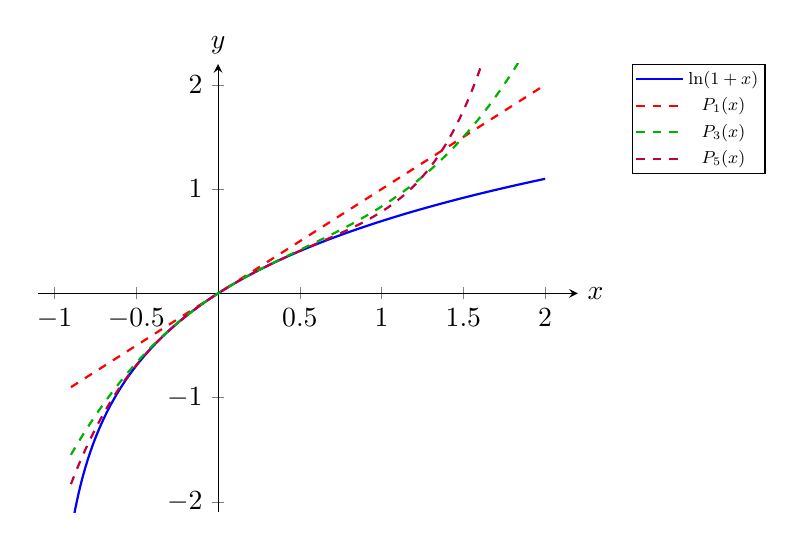
\begin{tikzpicture}
              \begin{axis}[
                  axis lines=middle,
                  xlabel={$x$},
                  ylabel={$y$},
                  x label style={anchor=west}, % label x ke kanan
                  y label style={anchor=south}, % label y ke atas
                  xmin=-1.1, xmax=2.2,
                  ymin=-2.1, ymax=2.2,
                  samples=200,
                  legend style={
                      at={(1.1,1)},
                      anchor=north west,
                      font=\small,         % mengecilkan ukuran font
                      row sep=1pt,         % jarak antar baris legend
                      inner sep=1pt,       % margin dalam kotak legend
                      nodes={scale=0.7}    % skalakan isi legend
                    }
                ]
                % fungsi asli
                \addplot[blue, thick, domain=-0.9:2] {ln(1+x)};
                \addlegendentry{$\ln(1+x)$}

                % P1
                \addplot[red, dashed, thick, domain=-0.9:2] {x};
                \addlegendentry{$P_1(x)$}

                % P3
                \addplot[green!70!black, dashed, thick, domain=-0.9:2] {x - x^2/2 + x^3/3};
                \addlegendentry{$P_3(x)$}

                % P5
                \addplot[purple, dashed, thick, domain=-0.9:2] {x - x^2/2 + x^3/3 - x^4/4 + x^5/5};
                \addlegendentry{$P_5(x)$}
              \end{axis}
            \end{tikzpicture}
          \end{center}
        \end{solusi}

  \item[\textbf{1.4}] \begin{itemize}
          \item[(i)] Tentukan sebuah polinomial
                \[
                  P(x) = \sum_{n=0}^{N} a_n x^n
                \]
                sedemikian sehingga
                \[
                  \left| \sin x - \sum_{n=0}^{N} a_n x^n \right| \leq 0.1,
                  \quad \forall x \in \left[0, \tfrac{\pi}{2}\right].
                \]
                \begin{solusi}
                  Polinomial Maclaurin untuk fungsi $\sin x$ adalah
                  \[
                    P_N(x) = \sum_{n=0}^{N} \frac{(-1)^n}{(2n+1)!} x^{2n+1} = x - \frac{x^3}{3!} + \frac{x^5}{5!} - \frac{x^7}{7!} + \cdots
                  \]
                  Cukup kita analisa $N$ yang memenuhi pertidaksamaan
                  \[
                    \frac{x^{2N+3}}{(2N+3)!} \leq 0.1, \quad \forall x \in \left[0, \frac{\pi}{2}\right].
                  \]
                  karena $x\leq \frac{\pi}{2}$, maka
                  \[
                    \frac{\left(\frac{\pi}{2}\right)^{2N+3}}{(2N+3)!} \leq 0.1.
                  \]
                  Dengan mencoba beberapa nilai $N$, diperoleh $N=1$ adalah yang paling kecil sehingga memenuhi pertidaksamaan di atas.
                  \[
                    \frac{\left(\frac{\pi}{2}\right)^{5}}{5!} = \frac{\left(\frac{\pi}{2}\right)^{5}}{120} \approx 0.0807 \leq 0.1.
                  \]
                  Jadi, polinomial yang diinginkan adalah
                  \[
                    P(x) = x - \frac{x^3}{6}.
                  \]
                  Selanjutnya akan coba kita perluas domain fungsinya menjadi $x\in[0,\pi]$. Dengan cara yang sama, kita peroleh
                  \[
                    \frac{\pi^{2N+3}}{(2N+3)!} \leq 0.1.
                  \]
                  Dengan mencoba beberapa nilai $N$, diperoleh $N=3$ adalah yang paling kecil
                  sehingga memenuhi pertidaksamaan di atas.
                  \[
                    \frac{\pi^{9}}{9!} = \frac{\pi^{9}}{362880} \approx 0.0926 \leq 0.1.
                  \]
                  Jadi, polinomial yang diinginkan adalah
                  \[
                    P(x) = x - \frac{x^3}{6} + \frac{x^5}{120} - \frac{x^7}{5040}.
                  \]
                  \begin{center}
                    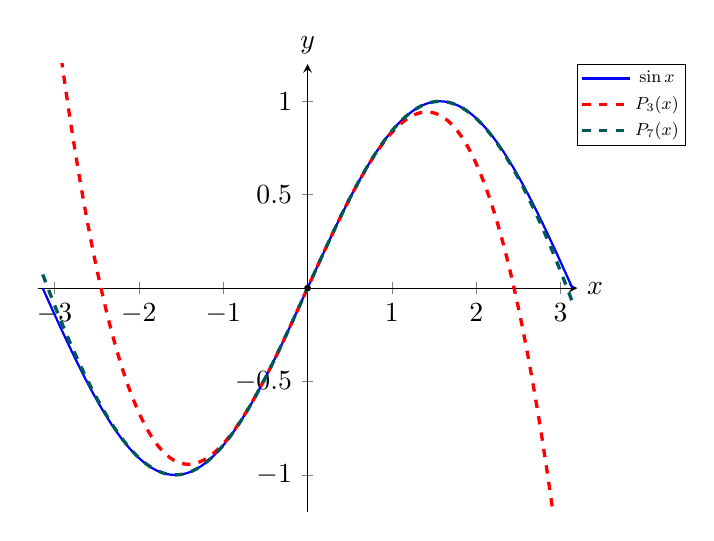
\begin{tikzpicture}
                      \begin{axis}[
                          domain=-3.14:3.14,    % -pi/2 .. pi/2
                          samples=300,
                          axis lines=middle,
                          xlabel={$x$},
                          ylabel={$y$},
                          x label style={anchor=west}, % label x ke kanan
                          y label style={anchor=south}, % label y ke atas
                          xmin=-3.2, xmax=3.2,
                          ymin=-1.2, ymax=1.2,
                          legend style={
                              at={(1,1)},
                              anchor=north west,
                              font=\small,         % mengecilkan ukuran font
                              row sep=1pt,         % jarak antar baris legend
                              inner sep=1pt,       % margin dalam kotak legend
                              nodes={scale=0.7}    % skalakan isi legend
                            }
                        ]

                        % sin x (exact)
                        \addplot[blue, thick] {sin(deg(x))}; % pgfplots expects deg() when using radian input in expression
                        \addlegendentry{$\sin x$}

                        % Maclaurin degree 3: x - x^3/6
                        \addplot[red, dashed, very thick] { x - (x^3)/6 };
                        \addlegendentry{$P_3(x)$}

                        % Maclaurin degree 7: x - x^3/6 + x^5/120 - x^7/5040
                        \addplot[teal!70!black, dashed, very thick] { x - (x^3)/6 + (x^5)/120 - (x^7)/5040 };
                        \addlegendentry{$P_7(x)$}

                        % optional: mark the origin
                        \addplot[mark=*, only marks, mark size=1pt] coordinates {(0,0)};

                      \end{axis}
                    \end{tikzpicture}
                  \end{center}
                \end{solusi}

          \item[(ii)] Gunakan hasil tersebut untuk mencari nilai hampiran dari
                \[
                  \int_{0}^{1} \sin(x^4)\, dx,
                \]
                dengan galat (error) paling banyak $0.1$.
                \begin{solusi}
                  Untuk $x\in[0,1]$ kita punya $x^4\in[0,1]\subset[0,\pi/2]$, sehingga
                  \[
                    \big|\sin(x^4)-P_4(x^4)\big| \le \frac{(\pi/2)^{5}}{5!}\approx 0.0796926,
                    \quad \forall x\in[0,1].
                  \]
                  Maka galat integral terbatasi oleh
                  \[
                    \left|\int_0^1\big(\sin(x^4)-P_4(x^4)\big)\,dx\right|
                    \le \int_0^1 0.0796926\,dx = 0.0796926 < 0.1.
                  \]

                  Hitung integral aproksimasi:
                  \[
                    \int_0^1 P_4(x^4)\,dx = \int_0^1\left(x^4-\frac{x^{12}}{6}\right)\,dx
                    = \frac{1}{5}-\frac{1}{78} = \frac{73}{390}\approx 0.1871795.
                  \]

                  Jadi diperoleh
                  \[
                    \int_0^1 \sin(x^4)\,dx \approx 0.1871795 \pm 0.1
                  \]
                \end{solusi}

        \end{itemize}
        \newpage
        \begin{center}
          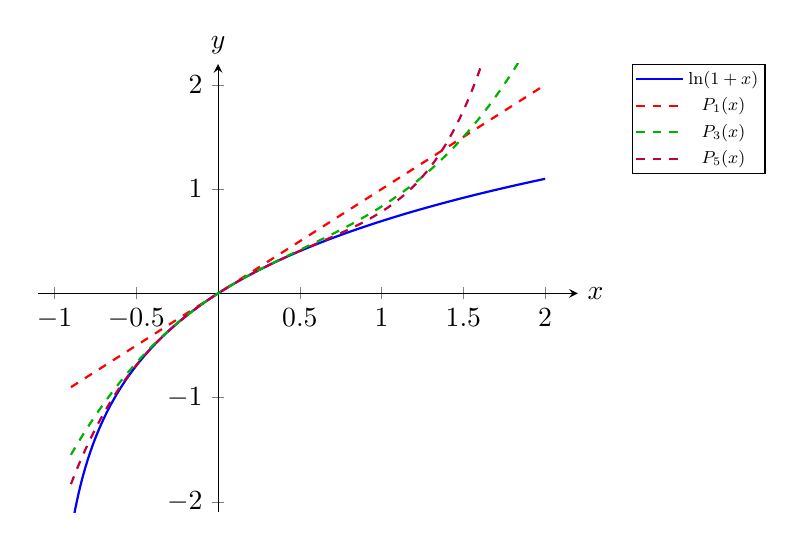
\begin{tikzpicture}
            \begin{axis}[
                axis lines=middle,
                xlabel={$x$},
                ylabel={$y$},
                x label style={anchor=west}, % label x ke kanan
                y label style={anchor=south}, % label y ke atas
                xmin=-1.1, xmax=2.2,
                ymin=-2.1, ymax=2.2,
                samples=200,
                legend style={
                    at={(1.1,1)},
                    anchor=north west,
                    font=\small,         % mengecilkan ukuran font
                    row sep=1pt,         % jarak antar baris legend
                    inner sep=1pt,       % margin dalam kotak legend
                    nodes={scale=0.7}    % skalakan isi legend
                  }
              ]
              % fungsi asli
              \addplot[blue, thick, domain=-0.9:2] {ln(1+x)};
              \addlegendentry{$\ln(1+x)$}

              % P1
              \addplot[red, dashed, thick, domain=-0.9:2] {x};
              \addlegendentry{$P_1(x)$}

              % P3
              \addplot[green!70!black, dashed, thick, domain=-0.9:2] {x - x^2/2 + x^3/3};
              \addlegendentry{$P_3(x)$}

              % P5
              \addplot[purple, dashed, thick, domain=-0.9:2] {x - x^2/2 + x^3/3 - x^4/4 + x^5/5};
              \addlegendentry{$P_5(x)$}
            \end{axis}
          \end{tikzpicture}
        \end{center}
        \begin{center}
          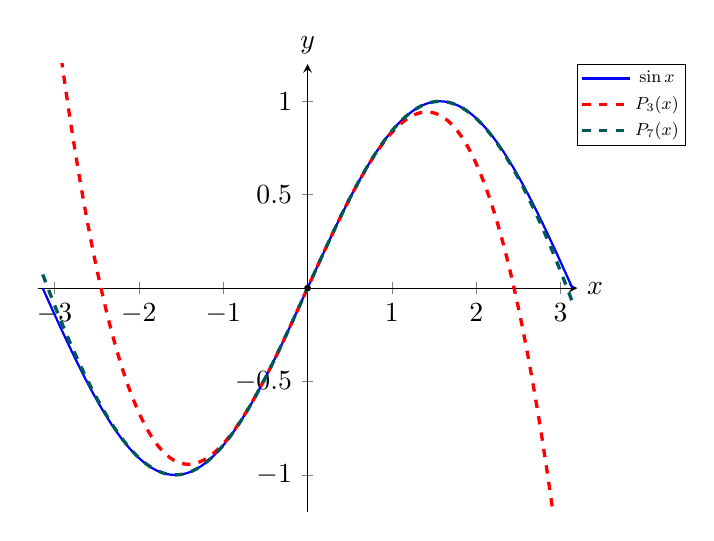
\begin{tikzpicture}
            \begin{axis}[
                domain=-3.14:3.14,    % -pi/2 .. pi/2
                samples=300,
                axis lines=middle,
                xlabel={$x$},
                ylabel={$y$},
                x label style={anchor=west}, % label x ke kanan
                y label style={anchor=south}, % label y ke atas
                xmin=-3.2, xmax=3.2,
                ymin=-1.2, ymax=1.2,
                legend style={
                    at={(1,1)},
                    anchor=north west,
                    font=\small,         % mengecilkan ukuran font
                    row sep=1pt,         % jarak antar baris legend
                    inner sep=1pt,       % margin dalam kotak legend
                    nodes={scale=0.7}    % skalakan isi legend
                  }
              ]

              % sin x (exact)
              \addplot[blue, thick] {sin(deg(x))}; % pgfplots expects deg() when using radian input in expression
              \addlegendentry{$\sin x$}

              % Maclaurin degree 3: x - x^3/6
              \addplot[red, dashed, very thick] { x - (x^3)/6 };
              \addlegendentry{$P_3(x)$}

              % Maclaurin degree 7: x - x^3/6 + x^5/120 - x^7/5040
              \addplot[teal!70!black, dashed, very thick] { x - (x^3)/6 + (x^5)/120 - (x^7)/5040 };
              \addlegendentry{$P_7(x)$}

              % optional: mark the origin
              \addplot[mark=*, only marks, mark size=1pt] coordinates {(0,0)};

            \end{axis}
          \end{tikzpicture}
        \end{center}
\end{enumerate}
\end{document}